\documentclass{article}

\usepackage{../mathclub}

\title{The Fundamental Group} 
\author{}
\date{February 28, 2022}

\begin{document}

\section{Introduction}
Welcome to Week 9 of Math Club! Today we'll be looking at some ideas in Topology, with a focus on the Fundamental Group! While normally this subject requires lots of technical machinery, we'll give a light introduction today that doesn't involve all the mind-bending definitions. That is, we will provide the intuitive idea behind these wonderful mathematical objects. Without further ado, doodoo.

\section{Not so rigorous definitions}
We will now introduce some very common topological spaces. 
\begin{center}
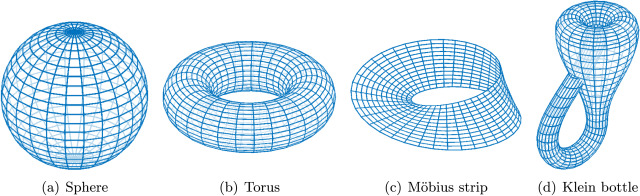
\includegraphics[scale=0.7]{Pics/sotrue} \quad 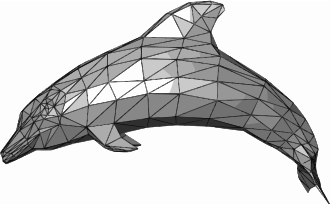
\includegraphics[scale=0.35]{Pics/dolp}\\
\end{center}
On first glance, all of these topological spaces look very different. However, proving that these topological spaces are actually 
\emph{topologically} distinct from each other is very nontrivial. For instance, how do you determine that a dolphin can't be ``morphed" into a pretzel? Now, we will introduce the idea of the Fundamental Group, one of many topological invariants. \\\\
\emph{Definitionoid} \\
We first familiarize ourselves with the notion of homotopic loops. Recall that a loop in some space $X$ is a continuous 
map $f: [0,1] \to X$, such that $f(0) = f(1)$. That is, imagine placing a piece of string onto some space (say a torus!) such that 
its ends are joined together. A homotopy of loops in $X$ is a family of loops $f_t$: $[0,1] \to X$ where $t \in [0,1]$, such that 
$f_t (0) = f_t(1)$ for all $t \in [0,1]$ and its associated map $F(s,t) = f_t (s)$ is continuous. Now imagine that the string is made out of rubber and you can stretch it around. The possible ``deformations" of our rubber string can be thought of as 
a homotopy class of loops. Now, we can talk about the Fundamental Group, $\pi_1 (X, x_0)$. Elements of the Fundamental Group are the
equivalence classes of homotopic loops with endpoints fixed at $x_0$. Intuitively, the Fundamental Group allows us to detect "holes" of a certain space (see torus). More importantly, it can be shown spaces with non-isomorphic Fundamental Groups must also be non-homotopic. \\\\
\emph{Formal definitions of the Fundamental group, higher order Homotopy groups, as well as singular/cellular Homology groups are available in
Algebraic Topology by Allen Hatcher. Probably also available on half of the internet.}
\\
\section{Exercises}
\begin{exercise}[Unsolved]
    Prove that dolphins are not homeomorphic to pretzels.
\end{exercise}
\begin{exercise}
    Convince yourself that the Fundamental Group of $\mathbb{R}^3$ is very trivial.
\end{exercise}
\begin{exercise}
    Convince yourself that the Fundamental Group of a coffee mug isn't too trivial. 
\end{exercise}
\begin{exercise} 
    Convince yourself that the Fundamental Group of a unit disk without origin isn't trivial.
\end{exercise}
\begin{exercise}
    Convince yourself that the Fundamental Group of $S^{1}$ is isomorphic to $\mathbb{Z}$.
\end{exercise}
\begin{exercise} 
    Convince yourself that the Fundamental Group of a sphere is trivial.
\end{exercise}
\begin{exercise} 
    Prove that $\pi_1 (S^n)$ is trivial for all $n > 1$.
\end{exercise}
\begin{exercise}
Let $X=\CC\setminus \{\pm 1\}$. Prove that $\pi_1(X)$ is not abelian.
\end{exercise}


\section{Homology}
As you may have realized, calculating the Fundamental group is \emph{fundamentally} a difficult problem (at least without a bit more tools). For higher dimensional spaces, calculating higher orders of Homotopy groups becomes ridiculously hard. Thus, Homology groups were created to remedy this issue. Here, we only give the definition of the simplicial homology. There are other notions of homology, like singular homology or cellular homology, and all of them are equivalent to each other under certain conditions. One may have a look at Hatcher's text to learn more about this. 

\begin{definition}
Let $a^{0}, \ldots, a^{n}$ be independent points in $\mathbb{R}^{m}$. Then, 
\[
\left\{\sum_{i = 0}^{n} \lambda_{i} a^{i}\mid \lambda_{i} \geq 0, \sum_{i = 0}^{n} \lambda_{i} = 1
\right\}
\]
is a $n$-simplex $\sigma^{n}$. A face $\tau$ of $\sigma$ is a simplex generated by some subset of the vertices, denoted by $\tau < \sigma$.  
\end{definition}

\begin{definition}
A simplicial complex $K$ is a finite set of simplices in some $\mathbb{R}^{n}$ so that 
\begin{itemize}
    \item $\sigma \in K$ and $\tau < \sigma$ implies that $\tau \in K$. 
    \item If $\sigma, \tau \in K$, then $\sigma \cap \tau = \emptyset$ or $\sigma \cap \tau$ is a face of both.  
\end{itemize}
\end{definition}

\begin{exercise}
Convince yourself that a $3$-simplex with its faces identified is just $S^3$. Or that $S^3$ is the union of two tori.
\end{exercise}

\begin{definition}
Let $\sigma^{n} = (a^{0}, \ldots, a^{n})$ be a $n$-simplex. There's an action of symmetric group $S_{n + 1}$ on vertices. Say that two simplices are equivalent if they differ by an even permutation. 
\end{definition}

\begin{remark}
It's not hard to see that the relation defined above gives an equivalence relation. An orientation of $\sigma$ is a choice of ordering.  
\end{remark}

\begin{definition}
A simplicial complex $K$ is oriented if a choice of orientations is made for its simplices. 
\end{definition}

\begin{definition}
Define the $n$-th chain group $C_{n}(K)$ of $K$ to be the free abelian group with one generator for each oriented simplex of dimension $n$. 
\end{definition}

\begin{definition}
Define the boundary homomorphism $\partial: C_{n}(K) \rightarrow C_{n - 1}(K)$ by 
\[
\partial[a^{0}, \ldots, a^{n}] = \sum_{i = 0}^{n} (-1)^{i} [a^{0}, \cdots \hat{a^{i}}, \ldots, a^{n}]. 
\]
\end{definition}

\begin{theorem}
$\partial^{2} = 0$. 
\end{theorem}

\begin{definition}
Set 
\begin{align*}
    Z_{n}(K) = \ker\{\partial_{n}: C_{n}(K) \rightarrow C_{n - 1}(K)\} 
\end{align*}
and 
\begin{align*}
    B_{n}(K) = \im\{\partial_{n + 1}: C_{n + 1}(K) \rightarrow C_{n}(K)\} 
\end{align*}
Elements of $Z_{n}(K)$ are called $n$-cycles while elements of $B_{n}(K)$ are called $n$-boundaries. By Theorem 4.1., $B_{n}(K)$ is a (normal) subgroup of $Z_{n}(K)$. So we define the $n$-th homology group of the chain complex to be the quotient group 
\[
H_{n} = Z_{n}(K)/B_{n}(K). 
\]
\end{definition}


\section{Further exercises}

\begin{figure}[hbt!]
\label{fig:aa}
\small
\centering
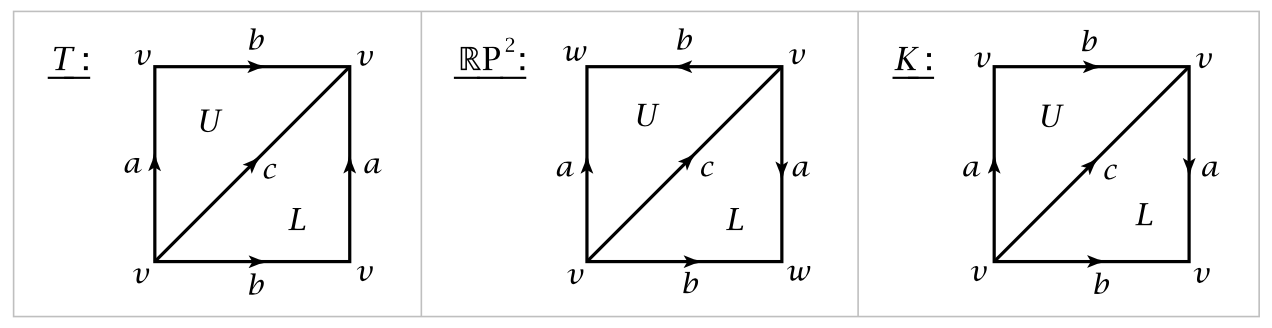
\includegraphics[scale = 0.5]{Pics/Simplicial.png}
\end{figure}
\leavevmode

\begin{exercise}
Compute the simplicial homology groups of $T$. 
\end{exercise}

\begin{exercise}
Compute the simplicial homology groups of the Klein bottle $K$.
\end{exercise}

\begin{exercise}
Compute the simplicial homology groups of $\mathbb{R}P^{2}$. 
\end{exercise}

\begin{exercise}
Let $X$ be the space obtained from $\mathbb{R}^{3}$ by removing the three coordinate axes. Calculate $\pi_{1}(X)$ and $H_{*}(X)$. 
\end{exercise}

\begin{exercise}
Let $L$ be a line in $\mathbb{R}^{3}$. Let $C$ be a round circle in $\mathbb{R}^{3}$ disjoint from $L$. Calculate the fundamental group of $\mathbb{R}^{3} - (L \cup C)$. Note that there are two cases to consider: one where the line goes through the interior of the circle, and the other where it doesn't. Are the spaces obtained in the two situations homotopy equivalent? 
\end{exercise}
\end{document}